\section{Методы решения начальных и краевых задач для обыкновенных дифференциальных уравнений (ОДУ) и систем ОДУ}

\subsection{Постановка задачи}
4.1. Реализовать методы Эйлера, Рунге-Кутты и Адамса 4-го порядка в виде программ, задавая в качестве входных данных шаг сетки $h$. С использованием разработанного программного обеспечения решить задачу Коши для ОДУ 2-го порядка на указанном отрезке. Оценить погрешность численного решения с использованием метода Рунге – Ромберга и путем сравнения с точным решением. 

{\bfseries Вариант:} 19
    \begin{equation}
        y'' + \frac{1}{x} y' + \frac{2}{x} y = 0, \\
        y(1) = 1, \\
        y'(1) = 1, \\
        x \in [1,2], h = 0.1
    \end{equation}
    
    \begin{equation}
		y = (cos(2)-sin(2))cos(2x^{1/2})+(cos(2)+sin(2))cos(2x^{1/2})
    \end{equation}
\pagebreak

\subsection{Результаты работы}
\begin{figure}[h!]
\centering
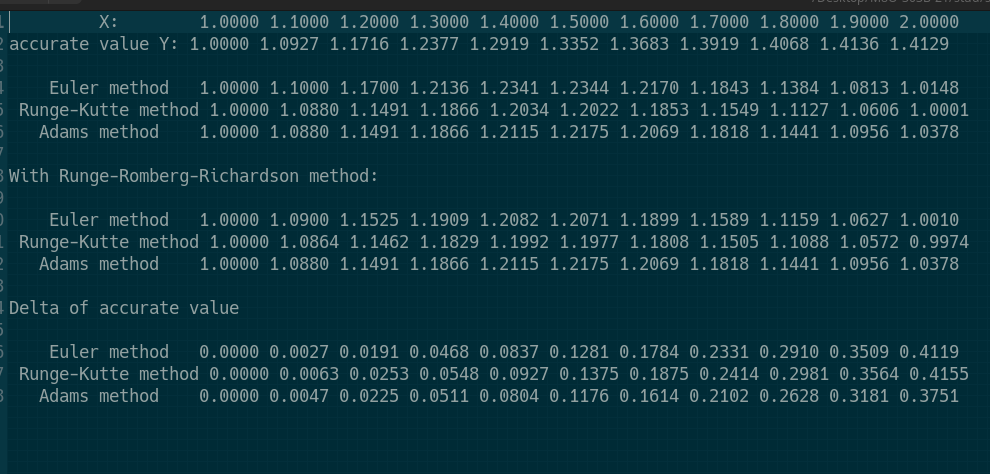
\includegraphics[width=.7\textwidth]{lab4.1}
\caption{Вывод в консоли}
\end{figure}


\subsection{Исходный код}
\lstinputlisting[title=\texttt{Lab4.1.cpp}]{../stud/saifullin/task4.1/Lab4.1.cpp}
\pagebreak

